\documentclass[10pt,a4paper]{article}
\usepackage[utf8]{inputenc}
\usepackage{amsmath}
\usepackage{amsfonts}
\usepackage{amssymb}
\usepackage{pgf-umlcd}
\usepackage{tabularx}
\usepackage{pdflscape}
\usepackage[obeyspaces]{url}
\usepackage{float}
\usepackage{framed}
\usepackage[linesnumbered]{algorithm2e}
\author{Myles Lee}
\title{Repository Knowledge Transfer in Automatic Optimisation of
Reconfigurable Designs}
\begin{document}

\maketitle
This project was supervised by Maciej Kurek and Wayne Luk and managed under the UROP scheme at the Custom Computing Group at the Department of Computing in Imperial College London.

\section{Introduction}
The objective is to optimise a design $T$, by finding the optimal configuration $\mathbf{x}_T^*$ using the performance metric $f_T$, using the least number of $f_T$ evaluations. $T$ has $n_T$ reconfigurable parameters, the design space $\mathbb{X}_T$ is defined to be the mathematical Cartesian product of $n_T$ intervals. $f_T$ is expensive to evaluate and cannot be assumed that $f_T$ is differentiable or convex. Therefore, computing $\mathbf{x}_T^*$ is expensive. Finding the true optimal design maybe too costly, and a sub-optimal configuration may be used.

Each design has a label function $g_T$, such that for some configuration $\mathbf{x}$, $g_T(\mathbf{x})=0$ if and only if $\mathbf{x}$ is successful. $g_T(\mathbf{x}_T^*)=0$ is required. In addition, each design have $m_T$ constraint functions $\{{h_1}_T,...\}$. Each constraint function determines the resource restrictions on the configurations. In the reconfigurable computing context, a constraint function could represent the fraction of a used hardware resource on the chip. For some constraint function ${h_i}_T$ and configuration $\mathbf{x}$, ${h_i}_T(\mathbf{x})<1$ if and only if $\mathbf{x}$ satisfies the $i^{th}$ constraint. Therefore $\forall \mathbf{x}\in\mathbb{X}_T.(\forall i\in\{1,...,m_T\}.{h_i}_T(\mathbf{x})<1)\Leftrightarrow g_T(\mathbf{x})=0$.

Moreover, each design have $c_T$ cost functions, where each cost function determines the cost of evaluating a component of $f_T$. For example, two cost functions can represent the software and hardware build time. The cost of evaluating $f_T(\mathbf{x})$ is the sum of each cost function, $\sum_{i=1}^{c_T}{c_i}_T(\mathbf{x})$. The cost of evaluating all samples may be minimised instead of minimising the number of evaluations, depending on the application of the optimisation.

To minimise this cost, a pre-optimised source design $S$ can be used to provide insight to a target design $T$ with limited sampling. Using observations from $f_S$, $\mathbf{x}_T^*$ can be approximated from $x_S^*$. Knowledge transfer is used to estimate properties of $T$ using other, possibility similar designs such as $S$. 

\section{Contributions}

The main contributions are summarised below:
\begin{enumerate}
\item Improvement of the surrogate to predict $f_T$, using a \emph{Transferable Gaussian Process}
\item Extension of knowledge transfer to predict optimal configuration at the first evaluation
\item Extension of knowledge transfer using multiple designs from a repository
\item Modification of previous code base\cite{Nicholson2015} with implementation of the above concepts
\end{enumerate}
\subsection{Transferable Gaussian Process}

Previous effort\cite{Kurek2016} used a polynomial function $z$ to map from source to target fitness values such that $z\circ f_S\approx f_T$. This is derived from linear regression of sampled source and target fitness values. However, $z$ is inaccurate for predicting when $f_S$ and $f_T$ are noisy or high dimensional functions. An example follows to demonstrate this.

Suppose $f_S(\mathbf{x})=1+\mathbf{x}_1$, $f_T(\mathbf{x})=1+\mathbf{x}_1+\mathbf{x}_2$ and $\mathbb{X}_S=\mathbb{X}_T=[0,1]^2$. By sampling at $\{(0,0),(0,1),(1,0),(1,1)\}$, we obtain the observations $\{((0,0),1),\allowbreak((0,1),1),((1,0),2),((1,1),2)\}$ and $\{((0,0),1),((0,1),2),((1,0),2),((1,1),3)\}$ by evaluating $f_S$ and $f_T$ respectively. By pairing source and target sample points, we obtain $\{(1,1),(1,2),(2,2),(2,3)\}$. Using linear regression, we can derive $z(y)=\frac{1}{2}+y$. Then for some sample, $(z\circ f_S)(x_1,x_2)=\frac{3}{2}+x_1\not=f_T(x_1,x_2)$. Therefore $z$ is inaccurate.

To solve this, a Transferable Gaussian Process (TGP) is used as follows. A TGP is composed of two Gaussian Processes of the same kernel, a process $p$ to predict the scalar of $f_S$ to $f_T$ and another process $q$ as a surrogate of $f_T$. $p$ is trained on the ratio of source and target fitness values, so $p(\mathbf{x})=\frac{f_T(\mathbf{x})}{f_S(\mathbf{x})}$ at sampled points. The training data for the example above would be $\{((0,0),1),((0,1),2),((1,0),1),((1,1),\frac{3}{2})\}$. $q$ is trained on observations of $f_S$, so $q=f_S$ at sampled points. Then we define $z(\mathbf{x})=p(\mathbf{x})q(\mathbf{x})$. So $(z\circ f_S)(\mathbf{x})=\frac{f_T(\mathbf{x})}{f_S(\mathbf{x})}\cdot f_S(\mathbf{x})=f_T(\mathbf{x})$. Using TGPs are more accurate than using polynomial regression because TGPs captures transferred features better in high dimensional space.

\subsection{Optimal Configuration Prediction}
Correlation analysis is used to determine the effectiveness of predicting the optimal configuration. For each dimension $i$ of the $\mathbb{X}_S$, we compute the Spearman correlation coefficient $\rho_i$ by comparing configurations against fitness values using observations of $f_S$. For a given significance level $\alpha$, if $\forall i\in\{1,...,n_S\}.1-|\rho_i|\le\alpha$ and $n_S=n_T$, then we can apply knowledge transfer. We approximate $f_S$ with a multi-dimensional quadratic function $\hat{f_S}$. We use multi-linear regression to find constants $c$, $\mathbf{d}$ and $\mathbf{e}$ such that $\hat{f_S}(\mathbf{x})=c+\sum_{i=1}^{n_S}\mathbf{d}_i \mathbf{x}_i+\mathbf{e}_i \mathbf{x}_i^2$. Then we approximate $\mathbf{x}_T^*=argmin_{\mathbf{x}\in\mathbb{X}_T}\hat{f_S}(\mathbf{x})$. This approximation is a signifiant improvement over using $\mathbf{x}_T^*\approx\mathbf{x}_S^*$ because $f_T$ and $f_S$ tend to be independent in each dimension and noisy\cite{Xi2004}. The evaluation illustrates this improvement.

\subsection{Repository Knowledge Transfer}

We know how to apply knowledge transfer from one design to another. To apply knowledge transfer from multiple sources, we need to select a design from the repository that has the highest transferability to optimise the target design. Formally, let the repository $R$ be the set of source designs $\{S_1,...\}$. Let $f_{transferability}$ measure the transferability of using knowledge transfer from $S$ to $T$. The objective is to find $argmax_{S\in R}f_{transferability}(S,T)$.

We extend designs to include parameter names and tags. For an arbitrary design $T$, parameter names $names_T$ label each element of a configuration. As different designs may share the same parameter names, we may be able to derive common properties of these designs. For example, when we decrease the width of mantissa widths in some design, we expect that this would generally reduce accuracy across any design. $T$ is associated with tags $tags_T$, which describes high-level keywords, such as ``uses square root" and ``implements matrix multiplication".

\[
	\begin{split}
		f_{transferability}(S,T)=f_{names}(S,T)\times(f_{common}(S,T)+f_{cross}(S,T)\\
			+f_{boundaries}(S,T)+f_{tags}(S,T))
	\end{split}
\] where
\[f_{names}(S,T)=|names_S\cap names_T|\]
\[f_{common}(S,T)=\text{number of common points in $O_S$ and $O_T$}\]
\[f_{cross}(S,T)=\text{leave-one-out cross-validation\cite{Jones1998} of predictor Gaussian process in TGP}\]
\[f_{boundaries}(S,T)=|\mathbb{X}_S\cup\mathbb{X}_T|/|\mathbb{X}_T|\]
\[f_{tags}(S,T)=|tags_S\cap tags_T|\]

The intuition of the definition of $f_{transferability}$ is derived by visualising designs on a hypergraph. Let a hypergraph $G$ have nodes for each unique name in any design of $R\cup\{T\}$. The hyperedges are the set of parameter names of each design $R\cup\{T\}$. If the hyperedges of two designs $S_1$ and $S_2$ intersect, then the number of intersecting nodes is $f_{names}(S_1,S_2)$. We only want to compare designs that have common names with $T$. Hence, $f_{names}(S,T)=0\Rightarrow f_{transferability}(S,T)=0$.

\subsection{Modification of Codebase}

For the full details of modifications, refer to the git repository of the accompanying source code. The main changes are summarised as below:
\begin{enumerate}
	\item Implement knowledge transfer
	\item Replaced particle swarm optimiser with a simplifed global Nelder Mead optimiser\cite{Luersen2004}
	\item Replace Python script interface with the Evaluator class that interfaces with arbitrary scripts
\end{enumerate}

The implementation of knowledge transfer follows the algorithm below. For the full details, see \path{transferrer.cpp}.
\begin{figure}[H]
	\begin{framed}
		\begin{algorithm}[H]
			Let $O_S$ and $O_T$ be observations from $S$ and $T$ respectively\\
			Filter $O_S$ if observation exceeds fitness percentile threshold $\beta$\\
			\If{$O_S$ is sufficently independent with significance level $\alpha$}{
				Compute multi-quadratic regression $\hat{f_S}$ from $O_S$\\
				$\mathbf{x}_q=argmin_{\mathbf{x}\in\mathbb{X}_S}\hat{f_S}(\mathbf{x})$\\
				$\mathbf{y}=(f_T(\mathbf{x}_q),g_T(\mathbf{x}_q),{h_1}_T(\mathbf{x}_q),...,{c_1}_T(\mathbf{x}_q),...)$\\
				Add $\mathbf{y}$ to $O_T$
			}
			Select $5n_T$ successful configurations randomly from $O_S$ into $\mathbf{X}$\\
			\For{$\mathbf{x}\in\mathbf{X}$}{
				$\mathbf{y}=(f_T(\mathbf{x}),g_T(\mathbf{x}),{h_1}_T(\mathbf{x}),...,{c_1}_T(\mathbf{x}),...)$\\
				Add $\mathbf{y}$ to $O_T$
			}
			Construct TGPs using $O_S$ and $O_T$\\
			Run EGO algorithm with TGPs
		\end{algorithm}		
	\end{framed}
	\caption{Single-source knowledge transfer algorithm}
\end{figure}

\section{Evaluation}

a load of graphs here

\section{Technical Documentation}

The program is written in C++ 14.

\subsection{Structure}

Below are files and directories in the working directory. 

\noindent
\begin{tabularx}{\textwidth}{|l|X|}
	\hline
	File/Directory & Description\\\hline
	animation & manages printing of animated progress to standard output\\\hline
	catch & unit test library\\\hline
	csv & manages file I/O to CSV files\\\hline
	compare & comparison metrics between source designs and a target design\\\hline
	eigen3 & libgp dependency\\\hline
	ego & efficient global optimiser\\\hline
	evaluator & interfaces command line script with runtime variables and caches results\\\hline
	examples & directory of designs used for benchmarking\\\hline
	functions & collection of general functions\\\hline
	gsl-2.4 & GNU scientific library\\\hline
	gp & wrapper for libgp's Gaussian process with log-space and whitening transformation\\\hline
	ihs & hypercube sampling library\\\hline
	logs & directory of experiment results and optimisation graphs\\\hline
	Makefile & builds and tests executable\\\hline
	tgp & implementation of TGP\\\hline
	transferrer & implementation of single knowledge transfer that wraps EGO\\\hline
	scripts & Bash and Python scripts to manage batch execution and manipulate CSV files\\\hline
	surrogate & interface for high dimensional regression\\\hline
\end{tabularx}
\begin{landscape}
	Below are scripts found in the scripts directory.
	
	\noindent
	\begin{tabularx}{\linewidth}{|l|X|X|}
		\hline
		Name & Description & Example\\\hline
		compare\_all\_experiments & runs program on all precomputed examples with and without knowledge transfer & \path{./scripts/compare_all_experiments}\\\hline
		compare\_experiments & runs program on source and target designs with and without knowledge transfer & \path{./scripts/compare_experiments examples/robot examples/stochastic 5}\\\hline
		compare\_kt.py & computes optimisation statistics from logs with and without knowledge transfer & \path{python3 scripts/compare_kt.py logs/robot_stochastic_no_kt.csv logs/robot_stochastic_kt.csv}\\\hline
		csv\_stats.py & computes statistics on a CSV file & \path{python3 scripts/csv_stats.py examples/robot/results.csv}\\\hline
		fill\_space.py & adds failed builds to precomputed results when results do not exhaustively represent the configuration space & \path{python3 scripts/fill_space.py examples/robot/results.csv 1 4 8 40}\\\hline
		interpolate.py & uses a Gaussian process to interpolate fitness values when results do not exhaustively represent the configuration space & \path{python3 scripts/interpolate.py examples/robot/results.csv examples/robot/config.txt 1 8}\\\hline
		parser.py & aggregates results by computing average fitness value of each duplicate sampled point & \path{python3 scripts/parser.py examples/robot/results.csv 2}\\\hline
		plot\_experiment.py & plots optimisation curve with and without knowledge transfer & \path{python3 scripts/plot_experiment.py logs/robot_stochastic_no_kt.csv logs/robot_stochastic_kt.csv}\\\hline
		plot\_predictions.py & plots 2-dimensional fitness function surface & \path{python3 scripts/plot_predictions.py examples/robot/results.csv output.png}\\\hline
		run\_example & runs program on a example design without knowledge transfer & \path{./scripts/run_example examples/robot}\\\hline
		transfer\_example & runs program on a target example design with knowledge transfer using a source & \path{./scripts/transfer_example examples/robot examples/stochastic}\\\hline
	\end{tabularx}
\end{landscape}
\begin{landscape}
	\noindent
	\begin{tabularx}{\linewidth}{|l|X|X|}
		\hline
		transfer\_repository & recommends a source example design for knowledge transfer of a target design & \path{./scripts/transfer_repository examples/robot}\\\hline
		transfer\_repository\_all & checks that all recommended source designs are most suitable for knowledge transfer across all example designs & \path{./scripts/transfer_repository_all}\\\hline
	\end{tabularx}
\end{landscape}

\begin{figure}[H]
	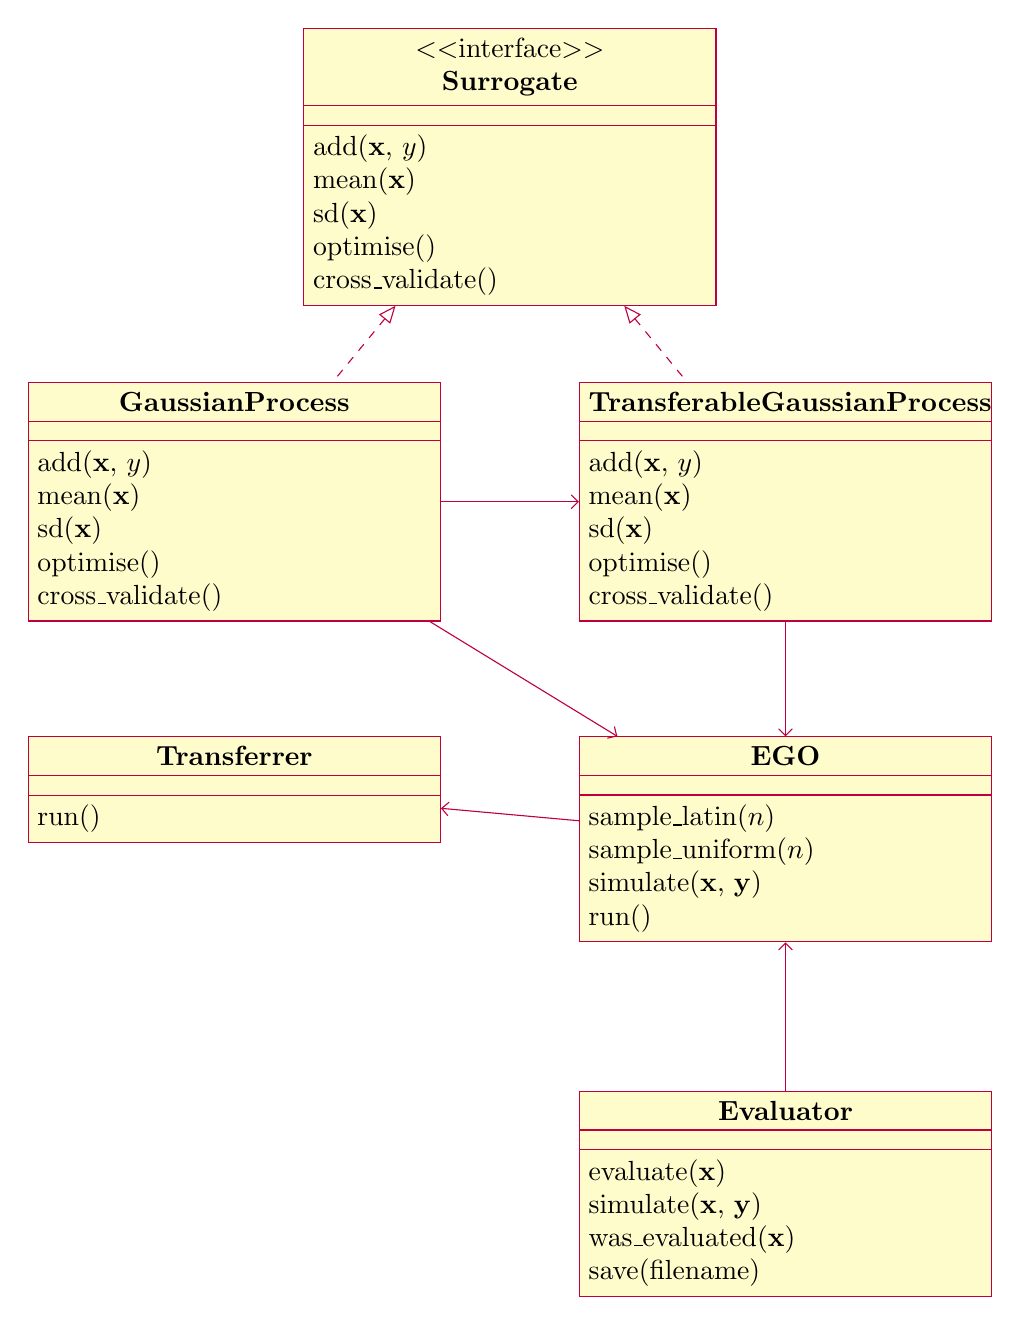
\begin{tikzpicture}
		\begin{interface}{Surrogate}{0 ,0}
			\operation{add($\mathbf{x}$, $y$)}
			\operation{mean($\mathbf{x}$)}
			\operation{sd($\mathbf{x}$)}
			\operation{optimise()}
			\operation{cross\_validate()}
		\end{interface}
		
		\begin{class}{GaussianProcess}{-3.5, -4.5}
			\implement{Surrogate}
			\operation{add($\mathbf{x}$, $y$)}
			\operation{mean($\mathbf{x}$)}
			\operation{sd($\mathbf{x}$)}
			\operation{optimise()}
			\operation{cross\_validate()}
		\end{class}
	
		\begin{class}{TransferableGaussianProcess}{3.5, -4.5}
			\implement{Surrogate}
			\operation{add($\mathbf{x}$, $y$)}
			\operation{mean($\mathbf{x}$)}
			\operation{sd($\mathbf{x}$)}
			\operation{optimise()}
			\operation{cross\_validate()}
		\end{class}
		
		\begin{class}{EGO}{3.5, -9}
			\operation{sample\_latin($n$)}
			\operation{sample\_uniform($n$)}
			\operation{simulate($\mathbf{x}$, $\mathbf{y}$)}
			\operation{run()}
	
		\end{class}
	
		\begin{class}{Transferrer}{-3.5, -9}
			\operation{run()}	
		\end{class}
	
		\begin{class}{Evaluator}{3.5, -13.5}
			\operation{evaluate($\mathbf{x}$)}
			\operation{simulate($\mathbf{x}$, $\mathbf{y}$)}
			\operation{was\_evaluated($\mathbf{x}$)}
			\operation{save(filename)}
		\end{class}
		
		\unidirectionalAssociation{GaussianProcess}{}{}{TransferableGaussianProcess}
		\unidirectionalAssociation{GaussianProcess}{}{}{EGO}
		\unidirectionalAssociation{TransferableGaussianProcess}{}{}{EGO}
		\unidirectionalAssociation{Evaluator}{}{}{EGO}
		\unidirectionalAssociation{EGO}{}{}{Transferrer}
	\end{tikzpicture}
	\caption{UML class diagram of program}
\end{figure}

\subsection{Design Specification}
For designs to be optimised by the program, each design must provide a configuration file and method to retrieve performance metrics. The configuration file defines the problem and determines how the program should interpret the results. A description of each configuration field is described below alongside the default configuration file.

\noindent
\begin{tabularx}{\linewidth}{|l|X|}
	\hline
	Configuration & Description\\\hline
	max evaluations & terminates program after number of $f_T$ evaluations exceed max evaluations\\\hline
	max trials & number of iterations for Monte-Carlo algorithms in the program that balances between configuration selection cost and evaluation cost\\\hline
	convergence\_threshold & terminates program when next evaluation is expected to improve less than the convergence threshold\\\hline
	discrete & \verb|false| when optimising real-valued configurations and \verb|true| when optimising integer-valued configurations\\\hline
	number of constraint functions & $m_T$\\\hline
	number of cost functions & $c_T$\\\hline
	lower boundaries & if $\mathbb{X}_T=[l_1,u_1]\times...\times[l_{n_T},u_{n_T}]$ then lower boundaries are $l_1,...,l_{n_T}$\\\hline
	upper boundaries & if $\mathbb{X}_T=[l_1,u_1]\times...\times[l_{n_T},u_{n_T}]$ then upper boundaries are $u_1,...,u_{n_T}$\\\hline
	significance level & negative transfer tolerance $\alpha$, when $\alpha=0$, knowledge transfer only occurs when $S$ has perfect correction with $T$, when $\alpha=1$, knowledge allows occurs\\\hline
	fitness percentile & fitness percentile threshold $\beta$, when $\beta=1$, use all samples, when $\beta=0.5$, only sample when fitness values are below the median, when $\beta=0$, do not use any samples\\\hline
	names & names for each configuration parameter transfer\\\hline
	tags & description of the design in keywords\\\hline
\end{tabularx}

\begin{figure}[H]
	\begin{framed}
		\begin{verbatim}
			# max evaluations
			1000
			# max trials
			100
			# convergence threshold
			0.0
			# discrete
			true
			# number of constraint functions
			0
			# number of cost functions
			0
			# lower boundaries
			0, 0
			# upper boundaries
			1, 1
			# significance level
			1.0
			# fitness percentile
			1.0
			# names
			
			# tags
			
		\end{verbatim}
	\end{framed}
	\caption{Default configuration file}
\end{figure}

Performance metrics can be either be generated through a script or be precomputed. The script takes $\mathbf{x}$ in the form of $n_T$ command line arguments and outputs $f_T(\mathbf{x}),g_T(\mathbf{x}),{h_1}_T(\mathbf{x}),...,{c_i}_T(\mathbf{x}),...$ as line-delimited values. Suppose $f_T(\mathbf{x})=\mathbf{x}_1+\mathbf{x}_2$ and $g_T(\mathbf{x})=\mathbf{x}_1$.

\begin{figure}[H]
	\begin{framed}
		\begin{verbatim}
			echo $(($1+$2))
			echo $1
		\end{verbatim}
	\end{framed}
	\caption{Example Bash script using default configurations}
\end{figure}

Suppose the configuration file was saved as \path{config.txt} and the script was saved as \path{script}. We can run the program with \path{./ego -o ./script config.txt output.csv}. The file \path{output.csv} contains the results of evaluating \path{script} with sampled points. This may be used as precomputed results.

When supplying precomputed results, the results are stored in a comma-delimited CSV without headers. Each row has $n_T+2+m_T+c_T$ cells. For some configuration $\mathbf{x}$, The first $n_T$ cells are $\mathbf{x}$, then $f_T(\mathbf{x})$, then $g_T(\mathbf{x})$, then each constraint ${h_i}_T(\mathbf{x})$, each ${c_i}_T(\mathbf{x})$. When $g_T(\mathbf{x})=0$, $x$ is successful, when $g_T(\mathbf{x})=1$, $x$ is unsuccessful and the program does not learn results, when $g_T(\mathbf{x})=2$, $x$ is unsuccessful but the program learns fitness values, constraints and costs. The difference between $g_T(\mathbf{x})$ being 1 or 2 depends on validity of the results. For example, if a configuration fails before performance metric can be measured, then rouge values should not be learnt.

\begin{figure}[H]
	\begin{framed}
		\begin{verbatim}
			0,0,0,0
			0,1,1,0
			1,0,1,1
			1,1,2,1
		\end{verbatim}
	\end{framed}
	\caption{Example precomputed result file using default configurations}
\end{figure}

Suppose the precomputed results file was saved as \path{results.csv}, then we can run the program with \path{./ego -o "python3 scripts/interpolate.py results.csv config.txt" config.txt}. The interpolation script wraps the results file into a script. Precomputed results can be used the script to reduce evaluations of the script by suppling the results as in \path{./ego -o ./script config.txt results.csv}.

\section{Future Work}

A limitation of the TGP is that only common points in the observations of $f_S$ and $f_T$ for the parameter Gaussian process are trained. When there are very few common points, the parameter Gaussian process predictions are inaccurate. A possible solution is to allow partial training of the Gaussian process by assigning a weight to each point. This weight would relate to the relative distance to the nearest common point. The implementation of this may require redesigning of the kernel, since the covariance matrix is parametrised by weights. Future work could investigate how TGPs can be improved.

\bibliographystyle{plain}
\bibliography{report}

\end{document}
